\chapter{Introduction}
\label{chp:introduction}
Tribler is a peer-to-peer file sharing program developed by the Delft University of Technology for research purposes.
Tribler expands the BitTorrent protocol and has added multiple improvements on this protocol.
The main focus of Tribler is to make security and privacy the default for Internet users
and make it impossible to shut the infrastructure of the Internet down.
A fully distributed program, not relying on any central component, is needed to achieve this.
Tribler has been designed and build using this methodology\cite{Pouwelse-tribler}\cite{Bakker-tribler}.
A distributed network requires collaboration of it peers to achieve success.
A schreenshot of Tribler can be seen in figure \ref{fig:tribler-schreenshot}
This master thesis was conducted as part of the research mission to improve the collaboration within Tribler.

\begin{figure}
	\centerline{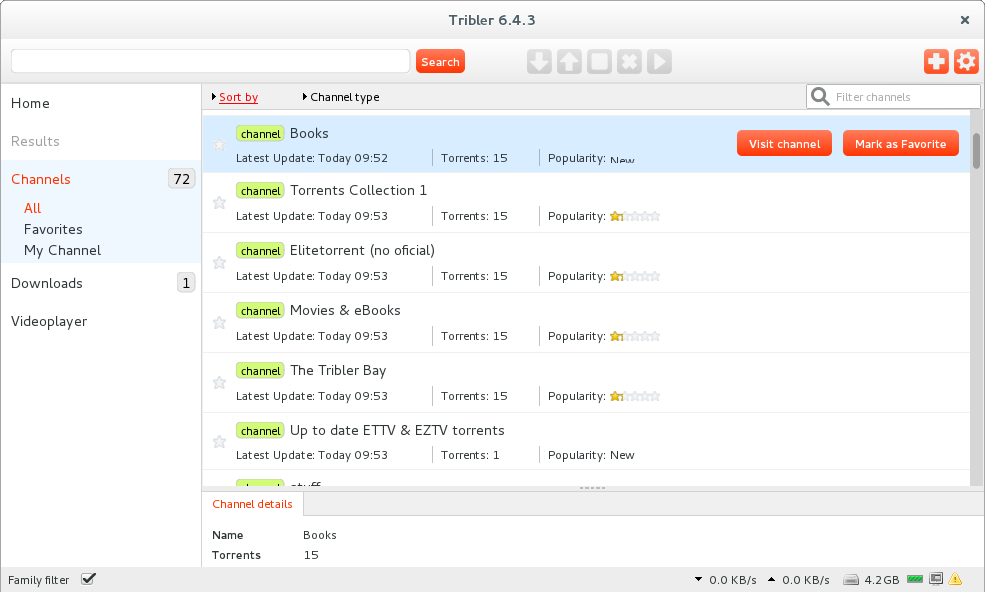
\includegraphics[scale=0.3]{introduction/figs/tribler-screenshot.png}}
	\caption{Schreenshot of Tribler v6.4.3.}
	\label{fig:tribler-schreenshot}
\end{figure}

\section{Tribler}
In peer-to-peer file sharing a node called a seeder uploads parts
of a file to another node, the downloader.
The role of being a seeder and downloader constantly changes
and a node can be both at the same time for different, parallel connections.
A seeder can become a downloader when they wish to download other files
and downloaders can become seeders,
if they posses a file someone else wants.
The ratio between the total size downloaded and uploaded is called the seeding ratio\cite{Cohen-bittorrent}.

The uploading can be seen as an interaction of one node helping another node.
These interactions comes at the cost of consuming bandwidth for both parties.
There is only direct benefit for the downloader.
The downloader receives a file he wants.
There is no direct barter between the seeder and downloader.
As the seeder does not get anything in return for uploading the file.
Although it can happen by chance that a downloader is also a seeder directly to the original seeder,
but this is unlikely\cite{Lai-Incentives}.

If everyone contributes, files become more available and are downloaded at higher speed.
This claim is supported by measurements taken in private communities
\cite{meulpolder-privatecommunities}.
In private communities high seeding ratio's are enforced by a tracker.
This tracker can be seen as a central, third party.
Both high availability and high download speeds result in a higher utility for the downloaders.
But currently freeriding in these networks takes places in high quantities\cite{Adar-Freeriding},
The BitTorrent Tit-for-Tat protocol is not enough to stop abuse\cite{Pouwelse-tribler}.

Tribler wants to achieve a high global seeding ratio by making it beneficial to have such a ratio.
Nodes can award each other with higher cooperation if a node has a reputation itself to be cooperative.
This requires for a tamper-proof interaction history to base a reputation on in a network.
Those contributing more receive more help in return,
and malicious nodes cannot abuse the network by tampering with the interaction history.

Tribler has recently implemented anonymous connections using onion routing \\\cite{Plak-anonymous}\cite{ruigrok-anonymous}.
This feature allows downloaders to become indistinguishable from other users in the network.
But every data packets has to be forwarded
by a number of intermediate hops between the downloader and seeder\cite{Plak-anonymous}.
The requirement of forwarding packets increases the network load of data being sent.
The total cost of bandwidth per file is increased,
but also the number of nodes helping a single node downloading a file increases.
This in turn increases the necessity of an incentive system to reward collaboration.

Dispersy is middleware for data dissemination in a network.
Dispersy is used heavily within Tribler and maintained by the Tribler organisation.
MultiChain is build upon Dispersy.
Dispersy can be used to exchange data between two specific nodes\cite{zeilemaker-dispersy}.
Improvements were added to Dispersy during the thesis.

\section{Document structure}
In chapter 1 we give an overview of what Tribler is and the organization that develops Tribler.
Chapter 2 gives a description of what the problem is of collaboration in peer-to-peer networks.
Chapter 3 provides an overview of related work of different approaches in solving the problem.
The design and implemention of the thesis work is described in chapter 4.
The implementation is tested and the experiments and results are described in chapter 5.
THe design has known vulnerabillities and these are explained in chapter 6.
Finally, we discuss the results of the work in chapter 7.
